\section{Matériels et méthodes}

\subsection{Cas d'étude}

La section \textit{Auricula} Duby du genre \textit{Primula} comprend 26 espèces et est endémique du système Alpin européen \citep{Ozenda1995}. Au sein de cette section, la sous-section \textit{Erythrodrosum} Pax englobe 7 espèces : \textit{P. villosa} Wulfen; \textit{P. daonensis} Leyb.; \textit{P. hirsuta} All.; \textit{P. apennina} Widmer; \textit{P. cottia} Widmer et \textit{P. pedemontana} Thom. ex. Gaudin. L'ensemble de ces espèces est ancestralement hexaploïde mais du fait de l'ancienneté de cet évènement de polyploïdisation, elles sont considérées ici comme diploïdes avec un nombre de chromosomes de x = 33. Leur niche écologique est située entre 1500 et 2500 mètres d'altitude (étages subalpins et alpins), et toutes sont spécialistes des substrats rocheux acides (fissures de rochers, éboulis et prairies alpines) \citep{Zhang2004}. La reproduction est allogame du fait d'une hétérostylie stricte, et a lieu au début du printemps après la fonte de la neige.

Leur répartition est soit très étendue (\textit{P. hirsuta}), soit restreinte à des massifs spécifiques et donc disjointe (Figure \ref{carte}). C'est le cas pour \textit{P. apennina, P. cottia et P. pedemontana}.

Concernant la population de \textit{P. pedemontana} des Écrins, la détermination est difficile, car les individus présentent diverses morphologies, dont une morphologie intermédiaire : une hampe proche de \textit{P. hirsuta} mais une pilosité semblable à \textit{P. pedemontana}. La morphologie foliaire est également variée au sein de cette population avec un bord plus ou moins denté selon les individus (lien web \ref{pne}).

\subsection{Échantillonnage}

Les données génétiques utilisées lors de cette étude ont été produites dans le cadre d'une étude précédente \citep{Boucher2016a}. Il s'agit d'un jeu de données composé de 90 individus de toutes les espèces composant \textit{Primula} section \textit{Auricula}, collectés entre avril et septembre 2014. L'identification taxonomique des individus a été réalisée sur le terrain, mais un individu a du être réattribué au taxon \textit{P. hirsuta} après analyse génétique.

Les individus avaient été génotypés dans le cadre d'une étude phylogénétique, avec le besoin de récolter de l'information sur l'ensemble du génome pour estimer une histoire phylogénétique non restreinte à un seul marqueur. À ces fins, l'ADN avait été génotypé par la méthode hyRAD \citep{Suchan2016} car cette technique permet de génotyper le long du génome malgré des mutations sur les sites de restrictions requis par les enzymes utilisées en RAD-seq \citep{Davey2010}. En effet les enzymes de restrictions utilisées en RAD-seq sont sensibles à la mutation d'un nucléotide, tandis que les sondes ARN utilisées pour la capture de \textit{loci} dans la méthode hyRAD peuvent s'hybrider sur ces sites de restriction RAD visés, même mutés. La nécessité de capturer des sites malgré une variance génétique provient du niveau interspécifique de l'étude, qui pose l'hypothèse que les mutations peuvent se placer sur les sites de restrictions et ainsi limiter leur capture par simple séquençage ddRAD. 

Les séquences obtenues par séquençage haut débit avaient été alignées sur le génome de référence de \textit{Primula veris} L. par le logiciel Bowtie2. Le jeu de données utilisé ('\verb|m13_-q20_mincov10|') est issu de divers filtres sur l'alignement, avec un score minimal de qualité (Phred) requis de 13 et une couverture minimale de 10 lectures par \textit{locus}. A partir de ces séquences, les SNPs ont été identifiées en utilisant Freebayes, avec un support de lecture de 30\% minimum par allèle, et ont été exportés sous format VCF.
\todo[color=blue!20]{Si besoin de place du peux enlever 'par le logiciel Bowtie2'}
%\todo[caption=reduc possible, color=yellow]{Si tu manques de place tu peux réduire toute cette section à quelques lignes seulement: tu est parti d'un jeu de données de SNPs pour 90 individus, obtenus après génotypage de type hyRAD et alignement sur un génome de réf.}

% extrait d'article de base :
%Total DNA was extracted from silica-dried leaves using a DNeasy Plant Mini kit (Qiagen, Hilden, Germany) following the manufacturer’s instructions. DNA quality was visualized on 0.8% agarose gels and quantity was assessed using a QuBit 2.0 fluorom- eter (2.0, Life Technologies, Carlsbad, CA, USA). Genomic DNA was converted into RAD-Capture genotyping-by-sequencing libraries (SNPsaurus, LLC), a new protocol aimed at harnessing the wide genomic spectrum of RAD-sequencing while reducing the amount of missing data in interspecific datasets. Briefly, a double-digest RAD library was created from 100 ng of a pool of genomic DNA containing a diverse set of individuals from sect. Auricula (belong- ing to P. allionii, P. apennina, P. auricula, P. glutinosa, and P. minima; see Table A.1). The pooled DNA was digested with PstI-HF and MfeI- HF (NEB) and ligated to complementary adapters that allowed the resulting amplified fragments to be converted to biotinylated RNA baits. Fragments with inserts roughly 100–350 bp in size were iso- lated by gel extraction from a portion of the ligated product prior to amplification and the in vitro transcription reaction to create the RNA baits. Shotgun sequencing libraries were prepared from the 90 study samples using 5 ng each in a 1/10th Nextera (Illumina, Inc) reaction with unique dual-indexes to distinguish the individu- als. The samples were pooled and size-selected for insert sizes roughly 170–370 bp. The pooled libraries were then used in two successive overnight hybridizations to the biotinylated bait library, followed by capture using DynabeadsÒ MyOneTM Streptavidin C1 magnetic beads (Thermo Fisher) and amplification. The final cap- tured products were sequenced in a single 150 bp NextSeq 500 High Output run at the Genomics and Cell Characterization Core of the University of Oregon.

%Therefore, varying the threshold on mapping quality allowed us to filter out ambiguously mapped reads that potentially represent multi-copy or repetitive regions of the genome (includ- ing paralogs) or are too divergent to be mapped to the reference genome reliably. We first applied a very stringent filter by only considering reads that mapped to the reference genome with a Phred quality score greater than 30, i.e. a mapping error rate lower than 0.1\% and with a coverage required to call a base higher than 20 in each sample (dataset ‘MAP30_COV20’). Since retaining only reads with a very high mapping quality to the reference genome might restrict our analyses to highly conserved regions of the gen- ome of primroses, we built a second dataset by retaining all reads with a mapping quality greater than a PHRED score of 13 (i.e. cor- responding to a 5% error rate in mapping) and with a coverage >10 in each sample (dataset ‘MAP13_COV10’). In a later step, indels, SNPs, and multiple nucleotide polymor-phisms were called with Freebayes (Garrison and Marth, 2012) using the BAM files of mapped reads from the two datasets. We used a minimum fraction of 30% of reads to support an allele, since in outcrossers like auriculas (Richards, 2003) we expect heterozy- gous loci to be common throughout the genome. Heterozygous positions were recorded using IUPAC ambiguity codes. We only called nucleotides with a base call quality greater than a Phred score of 20 (Freebayes parameters: ‘-q 20 -F 0.3’).

%\todo[inline,caption={mat met propre}]{Ici il faut prendre les choses dans l'ordre: tu ne peux pas commencer en disant 'les SNPs', on ne sait pas qu'ils existent. Idem pour le génome de référence: on ne sait pas à quoi il sert ici. Les grandes lignes logiques du génotypage c'est:
% 1) besoin d'avoir accès à de nombreuses régions du génome pour avoir un échantillon représentatif.
% 2) méthode RAD (dont il faut présenter le principe général) et dérivés OK, mais problème de perte d'allèles, surtout pour des données interspécifiques, d'où l'utilisation de capture hybride avec la méthode hyRAD.
% 3) séquençage et alignement des reads sur un génome de réf
% 4) SNP calling 
%Tu peux t'aider de mon papier pour ça bien sûr. Attention à ne pas laisser entendre que c'est toi qui a fait ces étapes 3 et 4 comme c'est un peu le cas ici. Pour plus de clarté tu pourrais sortir ça de ta partie 'Bioinfo'}

\subsection{Bioinformatique}

A partir du jeu de données initial, un pipeline est établi dans le langage R \citep{RTeam2017} pour générer divers ensembles de données, spécifiques à chaque analyse. Les fonctions sont rassemblées en un package R hébergé sur Github (lien web \ref{github}). Dans un premier temps, le fichier initial est traité avec la fonction \verb|subset_reorder|, qui permet de reconstruire le fichier en ne gardant que les individus souhaités dans l'ordre indiqué. Au maximum, les individus conservés à partir du jeu de donnée initial sont les individus de la sous-section \textit{Erythrodrosum} avec :
2 individus de \textit{P. apennina}, 
3 individus de \textit{P. cottia}, 
2 individus de \textit{P. pedemontana}, 
2 individus de \textit{P. pedemontana} des Écrins, 
6 individus de \textit{P. hirsuta}, 
4 individus de \textit{P. villosa}, 
2 individus de \textit{P. daonensis}.
Un individu de \textit{P. apennina} n'a pas été conservé comme dans l'étude de \citet{Boucher2016a}, car présentant trop de données manquantes. Toutes les informations concernant les individus de l'analyse sont présentées en annexe \ref{table_ind} et leur répartition est indiquée en Figure \ref{carte}.

La fonction suivante \verb|rare|, permet de trier les allèles considérés comme étant présents dans un trop faible pourcentage des individus. Ces allèles rares sont écartés du jeu de données et le locus pour l'individu présentant cet allèle rare est considéré comme une donnée manquante.

%\todo[inline,caption=rare,color = blue!20]{je ne sais pas si c'est l'approche standard, mais ça permet de garder l'information sur les autres individus. Au pire le \textit{locus} devient monomorphique. Et au pire si c'est une erreur, il se peut que le \textit{locus} ai un phred faible, et j'ai un seuil a plus tard pour ca.}

Cette étape permet également de supprimer les SNPs qui ont strictement plus d'un variant, qui sont reconnus comme des artefacts des algorithmes utilisés pour appeler les SNPs.
%We then filtered variants in a very conservative way by removing all called multiple nucleotide polymorphisms, indels and complex variants. These types of variants are known to often be artifacts generated by the algorithms used for short read mapping (see https://www. broadinstitute.org/gatk/guide/best-practices.php).
Afin de ne garder que les \textit{loci} polymorphes, nous utilisons ensuite la fonction \verb|clean|. Les \textit{loci} sont aussi filtrés sur le score de qualité (\verb|QUAL|) indiqué dans le vcf, qui correspond a la confiance dans l'assignation de l'allèle variant.
%In the context of variant calling, Phred-scaled quality scores can be used to represent many types of probabilities. The most commonly used in GATK is the QUAL score, or variant quality score. It is used in much the same way as the base quality score: the variant quality score is a Phred-scaled estimate of how confident we are that the variant caller correctly identified that a given genome position displays variation in at least one sample
 Une fonction nommée \verb|tri| est appelée pour supprimer les \textit{loci} puis les individus présentant trop de données manquantes selon les seuils posés. Enfin, afin de limiter le déséquilibre de liaison, les sites sont filtrés selon leur position sur les contigs du génome de référence: si deux SNPs sont situées à une distance inférieure à \verb|n| paires de bases, seul le premier est conservé.

Afin de pouvoir utiliser les fichiers triés sous divers formats, la sous-sélection d'individus et de \textit{loci} est enregistrée sous quatre formats (\verb|.vcf|, \verb|.str|, \verb|.geno|, \verb|.snp|) grâce à la fonction \verb|files|.
 La transformation d'un format en un autre se fait respectivement au moyen d'un script bash, par l'utilisation du software PGDSpider \citep{Lischer2012}, grâce au package LEA \citep{Frichot2015} et avec un script R.
\todo[color=blue!20]{Si besoin de place du peux enlever 'La transformation d'un format en un autre se fait respectivement au moyen d'un script bash, par l'utilisation du software PGDSpider \citep{Lischer2012}, grâce au package LEA \citep{Frichot2015} et avec un script R.'}

Toutes ces fonctions sont indépendantes mais peuvent être appelées dans l'ordre au moyen de la fonction \verb|dataset|, qui prend en entrée un vecteur de noms d'individus, un tableau contenant l'assignation de chaque individu à une population ou une lignée, le fichier \verb|vcf| original, le nom des fichiers de sortie et les seuils précisés au-dessus.

Chaque seuil est choisi après vérification que la décision n'impacte que peu les résultats de diversité génétique.
 Le nombre d'individus étant faible (22 au total), il faut optimiser le nombre de SNPs par individus car cela permet de limiter la perte d'information et d'atteindre les mêmes résultats qu'attendus avec un échantillon plus vaste \citep{Nazareno2017}.


\subsection{Génétique des populations}

Les analyses de génétique des populations ont été réalisées sous R avec différents packages. 
%\todo[color=blue!20]{\citep{RTeam2017}}

Dans un premier temps, des statistiques \verb|F| ont été calculées avec le package adegenet \citep{Jombart2011}. Ces statistiques permettent de se faire une première idée du jeu de données au niveau de la sous-section \textit{Erythrodrosum}, où le $F_{st}$ permet d'apprécier la présence d'une structure génétique entre les différentes populations.
 En parallèle, un clustering de nos individus a été réalisé afin d'essayer d'attribuer des groupes sans \textit{a priori}. Ce clustering fait par adegenet trouve les groupes pour lesquels la variance intergroupe est maximale quand la variance intragroupe est minimale. En plus de ce clustering, une analyse par composante principale discriminante a été réalisée pour visualiser la répartition des individus au sein des groupes.

Afin d'observer plus spécifiquement l'ensemble d'espèces de l'ouest des Alpes (\textit{P. hirsuta; P. apennina; P. cottia; P. pedemontana et P. pedemontana des Écrins}, nommé ci-dessous \clade{Hirsuta}), sa structure a ensuite été étudiée par le package LEA \citep{Frichot2015}. Cette structuration est établie par un algorithme sNMF, et permet d'estimer des coefficients d'admixture pour tout les individus. Pour cette étude, la structuration a été modélisée pour un nombre de groupes K allant de 2 à 5, avec 20 simulations par K et un alpha de 10, en ne retenant que la meilleure simulation basée sur le critère de "cross-entropy". Les structures avec K $>$ 5 ne sont pas étudiées, car le \clade{Hirsuta} ne contient que 5 taxons nommés, chacun n'étant représenté que par quelques individus seulement dans cet échantillonnage. Un K plus grand reviendrait à structurer ces lignées en assignant un individu par  groupe.

 %Une dernière mesure de génétique des populations a été réalisée pour essayer d'estimer l’expansion ou la contraction récente des populations par rapport . Ce \verb|D| de Tajima a été mesuré à l'aide du package pegas \citep{Paradis2010}.
 %\todo[inline]{Si tu inclus cette mesure il faut introduire avant à quoi celà va servir, sinon ça fait très 'exercice de style' en génét des pops. Tu pourrais évoquer les contractions de taille de population (efficace) pendant les cycles glaciaires en intro.}

%%%%%%%%%%%%%%%%  ABSENCE DE LA PARTIE DIYABC %%%%%%%%%%%%%%%%%

%\subsection{Inférences bayésiennes}

%Afin de caractériser l'admixture entre le taxon des Écrins et \textit{P. hirsuta}, une approche par approximate Bayesian computation (ABC) a été réalisée sur le logiciel DIYABC \citep{Cornuet2014}. Ce logiciel permet de simuler des jeux de données selon divers scénarios, en échantillonnant des paramètres entre des priors définis. Les scénarios sont ensuite classés selon les probabilités a posteriori d'observer notre jeu de donnée initial selon les scénarios proposés. Seuls quelques scénarios ont été étudiés ici, en prenant en compte le fait qu'ils sont à chaque fois supportés par peu d'individus. \todo[inline]{A reformuler, ce n'est pas une question de support des scénarios mais plutôt de taille du jeu de données en général.} Les priors sont également proposés dans un grand intervalle et selon une distribution uniforme, les temps de divergence entre populations et tailles de populations n'ayant pas ou peu été étudiés.

%Pour les topologies proposées en scénarios, toutes les topologies "classiques" sans évènement d'hybridation ont été proposées (5 cas possibles pour les 4 taxons composant  \textit{P. pedemontana s.l.}). Des topologies avec des polytomies regroupant plusieurs populations ont également été proposées. Enfin des hypothèses d'hybridation de \textit{pedemontana} et \textit{hirsuta} sont étudiées pour l'origine du taxon des Écrins.

%%%%%% mat&met thibaut coenonympha DIYABC %%%%%%
%with the approximate Bayesian computation (ABC) approach implemented in the software DIYABC (Cornuet et al. 2014). In short, a large number of simu- lated data sets were produced under each tested scenario by sampling parameter values into predefined prior dis-tributions, and an estimation of each scenario posterior probability was calculated as a function of the similarity between several summary statistics of simulated data sets and observed data using a logistic regression proce-dure. These posterior probabilities enable a ranking of scenarios and allow for the identification of the most probable evolutionary history. We only considered five evolutionary scenarios (Fig. 2), based on previously pub-lished studies dealing with the evolution of the complex (Porter et al. 1994; Wiemers 1998; Schmitt & Besold 2010) and our own hypothesis based on the morphometric and phylogenetic analyses (see Results). Scenario design and simulations. A uniform distribution with a large interval was chosen for each prior increas-ing the need in computation time but overcoming the lack of knowledge on population sizes, divergence times and admixture rate (see Table S2 Supporting information). Only one approximate C. arcania /C. gardetta divergence time of 1.5–4 million of years was available from Kodandaramaiah & Wahlberg (2009). For each scenario, a total of one million data sets were sim-ulated and the posterior probability was computed by performing a logistic regression on the 1% of simulated data closest to the observed data set (Cornuet et al.2008, 2010). Summary statistics used for observed/sim- ulated data sets comparisons are the mean gene diver-sity and Fst across all loci and Nei’s distances among populations. Gene diversity was chosen because allelic richness is directly influenced by hybridization; the genetic differentiation (Fst) and distance (Nei’s) among taxa were used because these indexes reflect the degree of differentiation between populations and are highly relevant to compare evolutionary histories. Assessing the ‘goodness of fit’ of the model. Once the most probable scenario was identified, different posterior anal-yses were carried out to evaluate the trustfulness of the procedure. First, to be sure of the choice of the scenario, 500 new data sets were simulated with each historical model creating pseudo-observed data sets for which pos-terior probabilities were re-estimated with the same pro-cedure described above. Type I and type II errors were evaluated by measuring, respectively, the fraction of data sets simulated under the best scenario that were assigned to other scenarios and the fraction of data sets simulated under other scenarios that were assigned to the best sce- nario. Second, we wanted to know whether our selected model is able to produce data sets similar to the observed one. This confidence in the model is evaluated by esti-mating the similarity between simulated (1000 simula-tions) and real data sets using summary statistics different than the ones used for model choice (an impor-tant precaution, see Cornuet et al. 2010). For each sum-mary statistic, a P-value is estimated by ranking the observed value among the values obtained with simu-lated data sets, and a principal component analysis was also performed to check visually the position of the observed data in relation to the data sets generated from the posterior predictive distribution. Posterior distribution of parameters and their precision. It was possible to evaluate the posterior distributions of parameters for our selected scenario using a local linear regression on the 1% of simulations closest to the observed data set (Cornuet et al. 2010). These distribu-tions gave an idea of the most probable value (median) and the ‘approximation’ (width of the distribution) for each historical model. A precision of these estimations was evaluated by computing the median of the absolute error divided by the true parameter value of the 500 pseudo-observed data sets simulated under the selected scenario using the median of the posterior distribution as point estimate (Cornuet et al. 2010).

\subsection{Hypothèse d'admixture}

Afin de tester l'hypothèse d'admixture pour le taxon des Écrins, un test "\verb|ABBA-BABA|" a été réalisé. Ce test d'admixture développé par \citet{Durand2011} propose une statistique (\verb|D|) basée sur quatre lignées partageant un ancêtre commun, selon la fréquence de SNPs observés avec un motif particulier sur une topologie de référence. 
% Cette méthode étant initialement pensée pour des séquences haploïdes. De fait la plupart des algorithmes présentés écartent les sites avec une ambiguïté (code IUPAC) ou alors résolvent l’ambiguïté par un tirage aléatoire entre deux bases. Il existe aussi une méthode pour prendre en compte les sites hétérozygotes à partir des fréquences alléliques, comme présenté dans \citet{Durand2011}, mais la faible taille de populations biaiserais les résultats. Il est donc plus judicieux d'écarter les sites hétérozygotes dans un premier temps, rendant le test plus conservateur.
% Considérant que les \textit{loci} sont sous une évolution neutre et sans déséquilibre de liaison, on attend deux configurations différentes pour une même topologie. 
Dans cette topologie, nous avons d'abord une divergence entre l'outgroup "O" et les autres taxons, suivie de la divergence de "P3" et finalement une divergence entre "P1" et "P2" (Figure \ref{abba-top}). 

Sur cette topologie on attend deux allèles présents en fin de branche avec "A" l'allèle ancestral et "B" l'allèle alternatif porté par certains individus de l'ingroup.
 Ce test ne s'intéresse qu'a deux cas : "ABBA" et "BABA", ce qui correspond à une minorité de \textit{loci}. Sous un modèle neutre, on attend des proportions équilibrées de \textit{loci} portant ces deux configurations. L'hypothèse alternative est qu'un déséquilibre de ces proportions peut être induit par une introgression de "P3" avec "P1" ou "P2". Une introgression entre "P3" et "P2" verrait donc une plus grande proportion de \textit{loci} à la configuration "ABBA" et une valeur positive du "\verb|D|" (Figure \ref{abba-top}).

\begin{figure}[!ht]
    \centering
    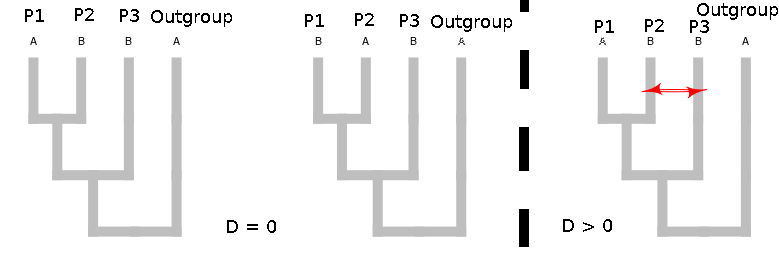
\includegraphics[width=1\textwidth]{fig/abba_mat.png}
    \caption{\textbf{Configurations d'allèles utilisées dans le test "ABBA-BABA".} Les deux schémas de gauche représentent les deux configurations d'allèles (respectivement "ABBA" et "BABA") en équilibre sous un modèle neutre (D=0).  Le schéma de droite montre un cas d'admixture entre "P1" et "P3", ce qui induit une plus grande proportion de la configuration schématisée (ABBA).}
    \label{abba-top}
    \centering
\end{figure} 
  %Cela aboutis à une valeur négative du "D", comme explicité par l'équation suivante :
% \[D(P1,P2,P3,0)=\frac{\sum_{i=1}^{n} C_{ABBA}(i)-C_{BABA}(i)}{\sum_{i=1}^{n} C_{ABBA}(i)+C_{BABA}(i)}\]
% Afin d'obtenir un résultat statistique, les individus sont tirés de manière aléatoire dans la population pour calculer la valeur de \verb|D|. Ce calcul est réitéré pour toutes les combinaisons possibles de tirage (dicté par les tailles de populations). 
% Devant le nombre réduit de sites informatifs avec rejet des sites hétérozygotes, 
Il a été décidé de calculer \verb|D| à partir des fréquences alléliques, comme décrit dans l'équation ci-dessous où \textit{$P_{ij}$} correspond à la fréquence de l'allèle alternatif (B).

\[D(P1,P2,P3,0)=\frac{\sum_{i=1}^{n} (1-P_{i1})P_{i2}P_{i3}(1-P_{i4})-P_{i1}(1-P_{i2})P_{i3}(1-P_{i4})}{\sum_{i=1}^{n} (1-P_{i1})P_{i2}P_{i3}(1-P_{i4})+P_{i1}(1-P_{i2})P_{i3}(1-P_{i4})}\]

Un intervalle de confiance sur cette statistique a été obtenu par bootstraping des SNPs, réalisé 1000 fois par échantillonnage aléatoire avec remise des \textit{loci}.
Il est important de souligner que ce test ne permet en aucun cas de proposer un sens d'introgression, ni son intensité. Afin de vérifier l'absence de faux positifs, ce test a été effectué avec des taxons pour lesquels aucune hypothèse d'admixture n'existe (\textit{P. apennina} et \textit{P. cottia}). De plus, pour ne pas biaiser l'analyse avec l'\textit{a priori} que le taxon des Écrins est issu d'une lignée de \textit{P. pedemontana}, l'admixture a été testé entre tout les taxons de \textit{P. pedemontana s.l.} et \textit{P. hirsuta}. Ce besoin de considérer toutes les entités taxonomiques présentes vient du fait que pour identifier la source de l'introgression, il faut considérer toutes les lignées dérivés de l'ancêtre commun \citep{Eaton2015}. Pour toutes les topologies différentes (voir \ref{ABBA} dans la partie résultat), \textit{P. daonensis} a été considéré comme l'outgroup, et \textit{P. hirsuta} comme P3. Ces choix découlent des résultats précédemment établis concernant la phylogénie de la sous-section \textit{Erythrodrosum} \citep{Boucher2016a}.

\iffalse % introgress n'est pas utilisé
\DIFdelend Une autre approche de l'admixture entre les taxons du \clade{Hirsuta} a été réalisée par le package introgress \citep{Gompert2010}, utilisé pour mesurer l'index h, index d'hybridation, entre \textit{P. pedemontana s.l.} et \textit{P. hirsuta}.
 Ce package requiert l'import des deux taxons parents présumés et des "hybrides" afin de mesurer un coefficient d'admixture (ou h-index) \DIFdelbegin \DIFdel{.
 Ce coefficient basé sur une fonction de vraisemblance \mbox{%DIFAUXCMD
\citep{Buerkle2005}}\hspace{0pt}%DIFAUXCMD
, où }\DIFdelend \DIFaddbegin \DIFadd{qui correspond à }\DIFaddend la proportion de chaque génome parental \DIFdelbegin \DIFdel{est mesurée dans }\DIFdelend \DIFaddbegin \DIFadd{\mbox{%DIFAUXCMD
\citep{Buerkle2005} }\hspace{0pt}%DIFAUXCMD
chez }\DIFaddend l'individu hybride.
\todo[inline,color=blue!20]{ça vaut peut être le coup de m'attarder sur comment il mesure ça. Si j'explique pas là et que j'ai a l'oral, je sais pas encore comment l'expliquer}
 Les marqueurs codominants utilisés ici n'étant pas tous fixés chez les parents, le calcul du h-index se basera ici sur les fréquences alléliques.
\fi